\section{Numerical Implementation}

This section describes the discrete fields, the transport--chemistry coupling,
and the per-timestep algorithm used in the reported simulations. The
implementation couples conservative Darcy-Brinkman-Stokes (DBS) transport
with cell-centred PHREEQC chemistry and cell-based surface complexation in a
single operator-split formulation.

\subsection{Field Locations And Discretization}

The discretization used throughout this paper keeps all chemistry-bearing state
cell-centered. The solution species, $\epsilon$ (denoted $\theta$ in the
analytical equations), $a_{\mathrm{surf}}$, and the adsorbed surface-species fields are stored at
cell centres, whereas the Darcy velocity $\bm{u}_D$ is face-centred. Transport
uses face interpolation within the conservative flux assembly, while surface
chemistry is evaluated as a cell-local update. The additive decomposition of
$a_{\mathrm{surf}}$ into interface and intrinsic contributions is defined in
Section~\ref{sec:aSurf}
(Eqs.~\eqref{eq:asurf}--\eqref{eq:asurf_intrinsic}).

All simulations reported here use the following discretization. Time
integration uses the first-order implicit Euler scheme, consistent with the
first-order Lie splitting of the transport and chemistry operators. The
convective term $\nabla\cdot(\bm{u}_D C_i)$ is discretized with the standard
first-order upwind scheme, which is bounded, monotone, and free of spurious oscillations
on the unstructured image-based meshes used here. The diffusive term
$\nabla\cdot(\theta D_i \nabla C_i)$ uses a second-order Gauss linear scheme
with non-orthogonality correction. The combination gives a scheme that is
first-order accurate in both time and space for advection-dominated transport,
consistent with the overall first-order operator-split framework.

\subsection{PHREEQC Coupling}

The PHREEQC coupling is selected with
\texttt{mixtureType phreeqcMixture} in
\texttt{constant/thermoPhysicalProperties}. This mixture wraps the PhreeqcRM
interface \citep{parkhurst2015phreeqcrm}. At
initialisation, each computational cell is registered as a separate PHREEQC
solution. When surface complexation is active, a PHREEQC \texttt{SURFACE}
block is also created for each reactive cell. For surface master $k$, its
capacity per representative bulk volume is
\begin{equation}
q_{\mathrm{sites},k} = s_k \, a_{\mathrm{surf}},
\label{eq:nsites}
\end{equation}
where $s_k$ (mol\,m$^{-2}$) is the user-prescribed site density for surface
master species $k$. This initialises the reactive capacity consistently with
the bulk-based surface-area field. PhreeqcRM is configured with its bulk
representative-volume surface convention, so no additional division by
porosity is applied.
The OpenFOAM dictionary stores $s_k$ in kmol\,m$^{-2}$, following the native
OpenFOAM amount unit; it is therefore multiplied numerically by $10^3$ when
interpreted as mol\,m$^{-2}$. Each surface-master density is supplied as an
OpenFOAM field, allowing spatially heterogeneous site densities.

The total $a_{\mathrm{surf}}$ field is computed before the simulation begins
(Section~\ref{sec:aSurf}), written as an OpenFOAM volume field, and read
explicitly by \texttt{reactiveTransportDBSFoam}. It is held constant throughout
the reactive-transport calculation; it is not updated by the flow or chemistry
solvers. The area and site capacity are transferred when the per-cell
PHREEQC surface templates are created and remain internal to PhreeqcRM during
the time loop. Consequently, the present implementation supports spatially
heterogeneous but time-independent $\epsilon$ and $a_{\mathrm{surf}}$; changing
either field during reactive transport would require rebuilding the PHREEQC
surface state. The surface mode is optional and reduces exactly to
aqueous-only mode when $a_{\mathrm{surf}} = 0$ everywhere.
For the image-based cases in this paper, a smooth sub-voxel reconstruction is
applied to the segmented occupancy field and the reconstructed
interface back into the CFD cells as volumetric $a_{\mathrm{surf}}$. In three
dimensions, \texttt{smoothSurface} extracts an isosurface and deposits the
resulting triangle areas into the cells that carry the reactive surface. In
quasi-two-dimensional image cases, it extracts an isoline on the image plane,
multiplies the reconstructed line length by the physical out-of-plane
thickness, and assigns the resulting area to the corresponding DBS cells. The
2D and 3D variants produce the same bulk field type and enter the same
cell-local PHREEQC mapping.

Cells with negligible mobile-water fraction
($\epsilon < \texttt{epsChemistryMin}$) are excluded from the fixed
finite-volume-to-PhreeqcRM mapping and do not contribute to chemistry.

The cell-local nature of the chemistry step means that all PHREEQC calls are
embarrassingly parallel across cells. PhreeqcRM distributes the cell
chemistry over available threads using OpenMP, so the chemistry cost scales
with the number of cores used for the transport solve.

\subsection{Per-Timestep Algorithm}

At startup, \texttt{reactiveTransportDBSFoam} reads the fixed porosity,
velocity, pressure, species, and explicit total surface-area fields. The
\texttt{phreeqcMixture} constructor then establishes a fixed mapping between
active finite-volume cells and PhreeqcRM cells. At each timestep, each aqueous
transport equation is advanced in conservative DBS form using the implicit
Euler--upwind discretization described above. The updated aqueous
concentrations and surface states are then pushed into PhreeqcRM, the local
equilibrium chemistry is evaluated for all active cells, and the updated
aqueous and surface concentrations are returned to the finite-volume fields.
The porosity and flow fields are not advanced in this PHREEQC mode. At
configured output times, OpenFOAM fields and a matching PhreeqcRM checkpoint
pair are written for chemically consistent restarts. Conservation is assessed
from the written fields using the domain-integrated bulk inventory
$M_{\mathrm{total}} = \sum_{\mathrm{cells}} V_{\mathrm{cell}}
\left( \theta C + a_{\mathrm{surf}}\Gamma \right)$
as a conservation diagnostic, where $V_{\mathrm{cell}}$ is the cell volume. In
a closed domain this quantity should remain constant to within discretisation
error; in a flow-through domain it should balance the net flux through the
inlet and outlet faces.

The operator-split structure keeps
transport and chemistry individually testable and ensures that the
conservative structure of the aqueous transport step is not hidden inside a
composite implicit source term.

\begin{figure}[htbp]
    \centering
    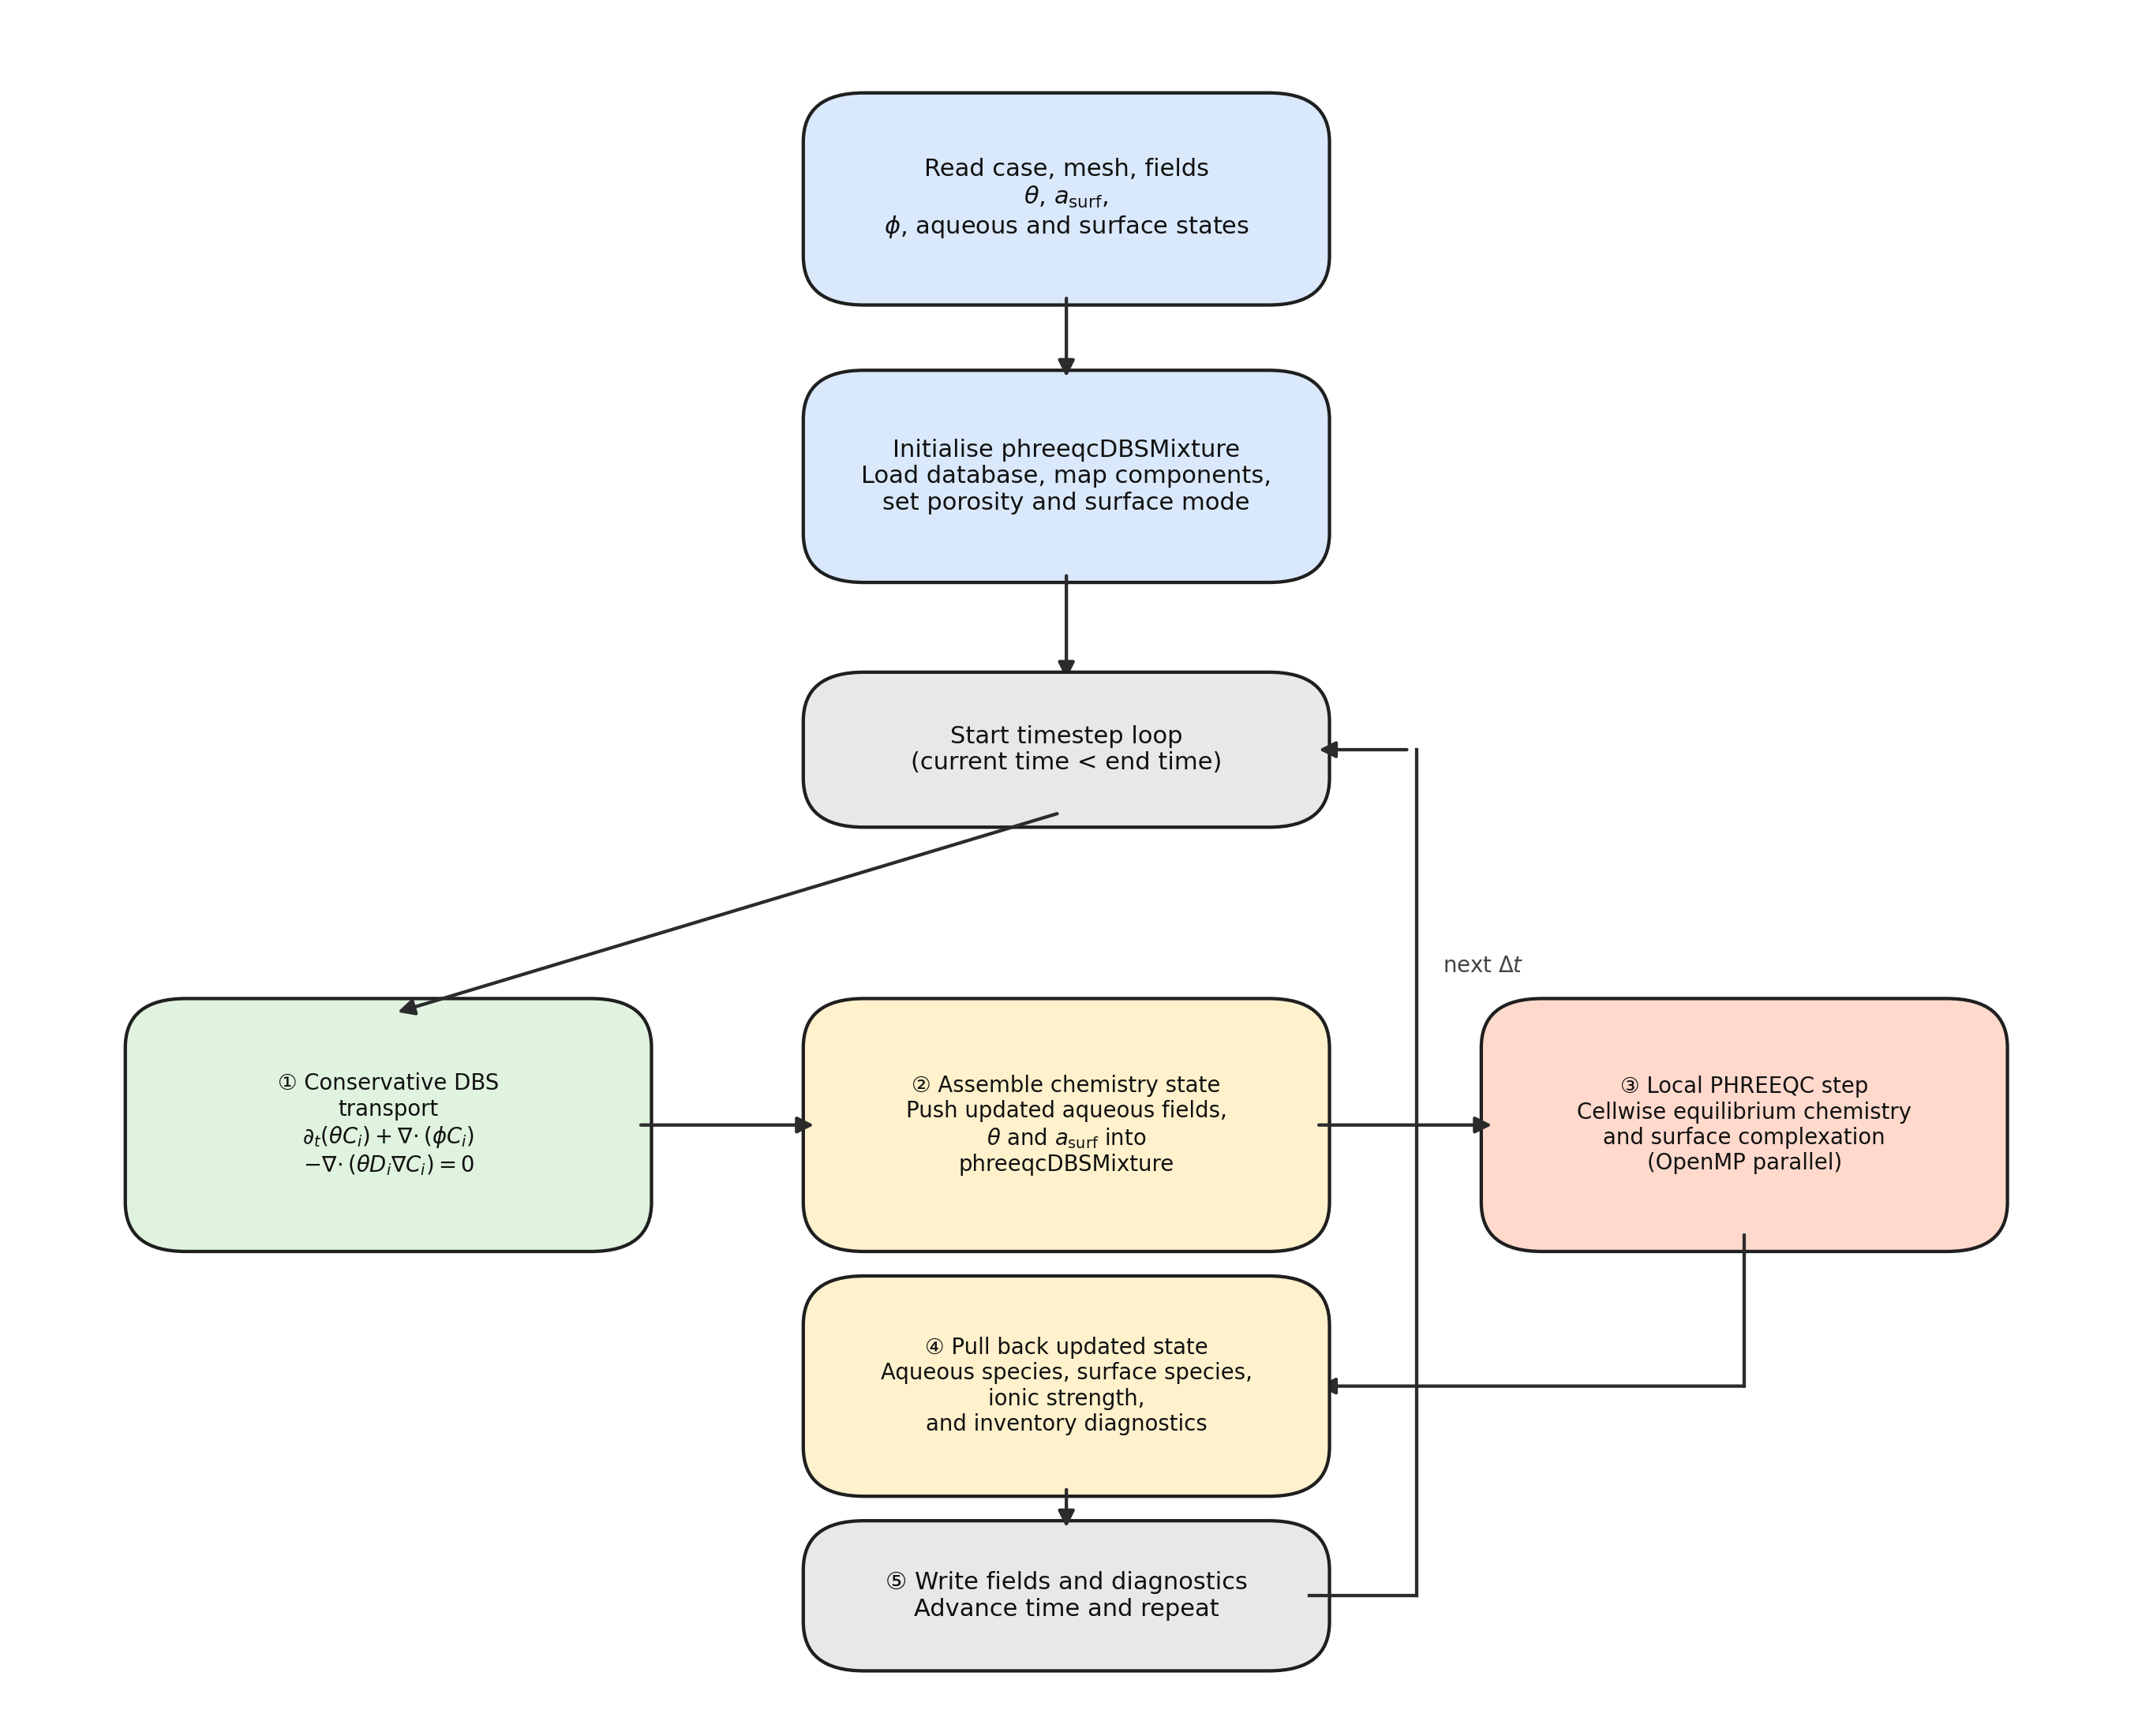
\includegraphics[width=0.96\linewidth]{figures/png/fig05_solver_workflow.png}
    \caption{Full solution procedure for
    \texttt{reactiveTransportDBSFoam}. The solver reads the current
    finite-volume state, initializes or updates the cell-based PHREEQC
    coupling through \texttt{phreeqcMixture}, advances all aqueous species
    in conservative DBS form, executes the local cellwise chemistry update,
    and then writes the updated aqueous and surface states back to the
    finite-volume fields. The workflow is intentionally operator-split:
    transport is solved first, followed by local PHREEQC chemistry, so the two
    operators remain independently testable and the conservative structure of
    the aqueous transport step is never hidden inside an implicit composite
    source term.}
    \label{fig:dbsWorkflow}
\end{figure}

Figure~\ref{fig:dbsWorkflow} illustrates the implemented algorithm. Solver
selection is made through \texttt{mixtureType}: the surface-complexation cases
use \texttt{phreeqcMixture}, whereas the upstream kinetic-mineral formulation
uses \texttt{inertMultiComponentMixture}. The chemistry state remains
cell-centred throughout the loop. The solver does not
convert the unresolved surface reaction into an equivalent face flux. Instead,
transport acts through the aqueous face fluxes, while PHREEQC updates the
cell-local aqueous and adsorbed inventories after each transport solve.
